\section{Dataset Analysis}
\label{sec:dataset_analysis}

We introduce the MultiEMiT corpus, a multi-layered multimodal dataset of Italian Twitter commentary gathered during live television broadcasts. The data originates from the M.EMO.RAI project \cite{memorai}, which set out to track audience emotional responses in real time. Rather than restricting annotations to positive or negative sentiment, MultiEMiT applies an expanded eight-emotion taxonomy derived from Plutchik's psychoevolutionary model \cite{Plutchik}.

MultiEMiT was collected from two television broadcasts, representing contrasting formats and registers:

\textit{ProSAT:} Twitter commentary on \textit{Propaganda Live}, a satirical talk show on LA7 combining investigative journalism and political commentary \cite{propagandalive}. The collection captures the broadcast of November 19, 2021, when host Diego Bianchi reported live from the Poland-Belarus border during a humanitarian crisis. The gravity of the event prompted solemn reactions dominated by indignation, grief, and civic debate.

\textit{EMiT (Pechino Express):} Inspired by the EVALITA 2023 EMiT benchmark \cite{emit}, this sub-corpus covers \textit{Pechino Express}, an adventure reality show broadcast on Rai2 \cite{pechinoexpress}. Collected during the season premiere on February 11, 2020, viewer discourse centers on lighthearted entertainment, contestant rivalries, and humorous commentary.

Both collections share an identical structure: a purely textual partition and a multimodal partition pairing the text with its attached media (screenshots, edited images, and memes). This paired structure allows direct comparison between unimodal and multimodal models, showing where visual content modulates the written post. In addition to MultiEMiT, two external Italian textual corpora are used as supplementary training data only: EVALITA 2023 EMiT (5,966 posts across multiple programs \cite{emit}) for emotion detection and IronITA (4,849 posts \cite{ironita2018}) for irony detection.

Annotation was conducted on Sensitag, a web annotation platform developed at the University of Turin. Each post was evaluated independently by three annotators with backgrounds in computer science or linguistics. Final labels were assigned by majority vote (at least two out of three annotators agreeing) to create a golden dataset.

\begin{figure}[!t]
\centering
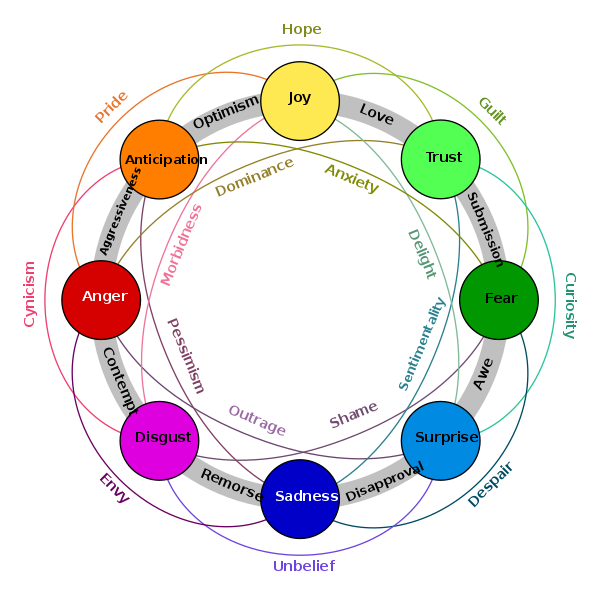
\includegraphics[width=0.88\columnwidth]{imgs/Plutchik_Dyads.svg.png}
\caption{Robert Plutchik's psychoevolutionary emotion schema \cite{Plutchik} and derived affective dyads. Primary emotional axes arranged along the perimeter combine systematically into secondary and tertiary affective blends (e.g., \textit{Joy} + \textit{Trust} yields \textit{Love}, while \textit{Disgust} + \textit{Anger} yields \textit{Contempt}).}
\label{fig:plutchik_dyads}
\end{figure}

The corpus is annotated across five pragmatic dimensions:
\begin{itemize}
    \item \textbf{Emotions:} Ten affective categories grounded in Plutchik's psychoevolutionary model \cite{Plutchik} (\textit{Joy}--\textit{Sadness}, \textit{Trust}--\textit{Disgust}, \textit{Fear}--\textit{Anger}, \textit{Surprise}--\textit{Anticipation}), supplemented with \textit{Love} and \textit{Neutral}. According to Plutchik's theory, primary emotional axes combine systematically along the wheel into complex secondary and tertiary affective states, termed \textit{dyads} (e.g., \textit{Trust} + \textit{Joy} = \textit{Love}, \textit{Disgust} + \textit{Anger} = \textit{Contempt}, \textit{Sadness} + \textit{Disgust} = \textit{Remorse}, or \textit{Anger} + \textit{Surprise} = \textit{Outrage}), as illustrated in Fig.~\ref{fig:plutchik_dyads}. This combinatory nature provides theoretical justification for formulating emotion detection as a multi-label task \cite{mohammad2018semeval, demszky2020goemotions}, allowing social media posts to express complex or multiple emotions.
    \item \textbf{Irony and Sarcasm:} Three exclusive classes separating literal statements (\textit{Unironic}), humorous figurative inversion (\textit{Irony}), and hostile, denigratory mockery (\textit{Sarcasm}).
    \item \textbf{Offensiveness:} A binary indicator identifying abusive language, insults, or harassment directed at individuals or protected groups (incorporating rare hate speech instances due to their scarcity in broadcast commentary; all remaining posts are non-offensive).
    \item \textbf{Target:} Distinguishes whether comments address the broadcast \textit{Content} (political issues, guests, or news events) or the \textit{Container} (the studio host, network, or production execution). Because posts may use the broadcast hashtag without referencing the program itself, or comment on both aspects at once, a post can have no target (292 textual and 58 multimodal posts) or both targets simultaneously (61 textual and 7 multimodal posts).
    \item \textbf{Semiotic Relation:} Categorizes multimodal document intent based on the semiotic taxonomy established by Kruk et al. \cite{MultiM} into three foundational relationships (depicted in Fig.~\ref{fig:semiotic_relations}): \textit{Additive}, where text and image mutually enrich and expand each other to produce a cohesive narrative; \textit{Parallel}, where both text and visual media redundantly express the same semantic information independently; and \textit{Divergent}, where textual and visual cues convey contrasting or incongruent signals, creating cognitive dissonance, ironic tension, or meme subversion.
\end{itemize}

\begin{figure*}[!t]
\centering
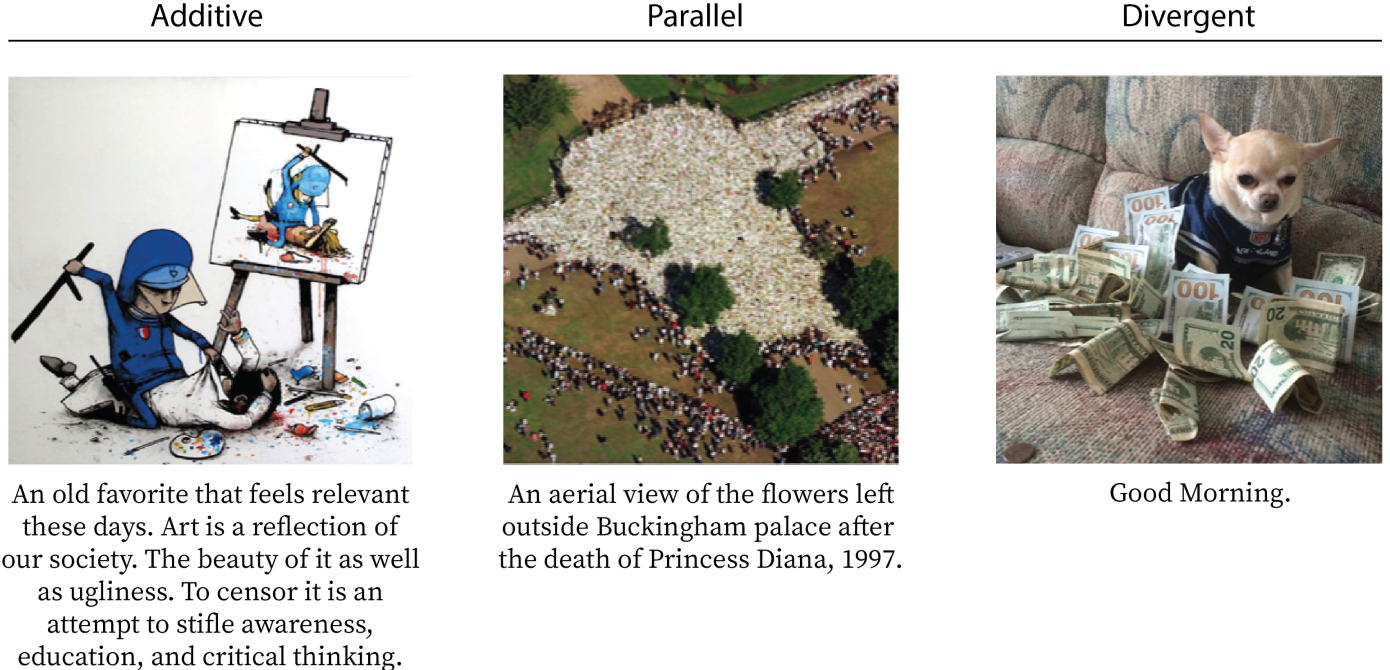
\includegraphics[width=0.92\textwidth]{imgs/Additive_divergent_parallel.png}
\caption{Taxonomy of semiotic text--image relationships defined by Kruk et al. \cite{MultiM}: \textit{Additive} (text and image mutually enrich one another to produce new contextual depth), \textit{Parallel} (both modalities independently deliver redundant semantic meaning), and \textit{Divergent} (semantic or pragmatic conflict between modalities, generating irony, cognitive tension, or satirical contrast).}
\label{fig:semiotic_relations}
\end{figure*}

\begin{figure}[!t]
\centering

\includegraphics[width=0.95\columnwidth]{imgs/interpretation_of_posts.png}
\caption{Example of an ambiguous Social TV post from the \textit{Propaganda Live} collection evaluated by three independent annotators. Despite viewing identical multimodal content, each annotator assigned a distinct emotional reading (\textit{Anger}+\textit{Disgust} vs. \textit{Sadness}+\textit{Surprise} vs. \textit{Disgust}+\textit{Fear}), illustrating the inherent difficulty of human agreement in subjective affective tasks and the pruning effect of majority-voting gold standard consolidation.}
\label{fig:interpretation_of_posts}
\end{figure}

Emotions in short social media commentary are inherently ambiguous, and human annotators frequently diverge in their subjective interpretations. Figure~\ref{fig:interpretation_of_posts} illustrates a compelling example from the \textit{Propaganda Live} collection, where the post \textit{``Terrible, I'm ashamed of being European''} was paired with broadcast stills of shivering refugee families at the Poland--Belarus border. Despite reading the exact same text and inspecting the same imagery, the three independent annotators arrived at three distinct emotional interpretations:
\begin{itemize}
    \item \textit{Annotator 1} marked \textit{Anger} and \textit{Disgust}, interpreting the post as indignant moral outrage toward European governance;
    \item \textit{Annotator 2} selected \textit{Sadness} and \textit{Surprise}, reading it as shocked disbelief and disapproval;
    \item \textit{Annotator 3} chose \textit{Disgust} and \textit{Fear}, capturing internalized shame and apprehension.
\end{itemize}
Under our strict majority-voting protocol (which requires agreement from at least two out of three annotators to retain a label in the golden dataset), only the overlapping label \textit{Disgust} was preserved, while the distinct yet plausible secondary interpretations were pruned. This example vividly underscores the challenge of achieving human annotator consensus on subjective social media tasks \cite{demszky2020goemotions, basile2021disagreement}.

\begin{table}[!t]
\centering
\caption{Inter-Annotator Agreement (Fleiss' $\kappa$) across Pragmatic Dimensions and Multimodal Disambiguation Gain on Paired Posts ($N = 628$)}
\label{table:fleiss_kappa}
\footnotesize
\setlength{\tabcolsep}{2.5pt}
\renewcommand{\arraystretch}{1.05}
\resizebox{\columnwidth}{!}{%
\begin{tabular}{l | c c | r}
\hline
\textbf{Pragmatic Dimension} & \textbf{Text-Only} & \textbf{With Image} & \textbf{Visual Gain} \\
\textbf{/ Category} & \multicolumn{2}{c|}{\textbf{(Paired $N = 628$)}} & \textbf{($\Delta\kappa$ / \%)} \\
\hline
\multicolumn{4}{l}{\textit{Emotions (Plutchik)}} \\
\hline
Love & 0.270 & 0.159 & $-0.111$ ($-41.2$\%) \\
Anticipation & 0.469 & 0.573 & +0.104 (+22.3\%) \\
Disgust & 0.518 & 0.522 & +0.005 (+0.9\%) \\
Trust & 0.444 & 0.515 & +0.072 (+16.1\%) \\
Joy & 0.451 & 0.390 & $-0.062$ ($-13.7$\%) \\
Fear & 0.172 & 0.215 & +0.043 (+24.7\%) \\
Anger & 0.353 & 0.454 & +0.101 (+28.5\%) \\
Surprise & 0.246 & 0.255 & +0.009 (+3.7\%) \\
Sadness & 0.272 & 0.312 & +0.039 (+14.5\%) \\
Neutral & 0.274 & 0.359 & +0.085 (+31.0\%) \\
\hline
\textbf{Emotion Level Mean} & \textbf{0.347} & \textbf{0.375} & \textbf{+0.028 (+8.2\%)} \\
\hline
\multicolumn{4}{l}{\textit{Irony and Sarcasm}} \\
\hline
Irony & 0.426 & 0.596 & \textbf{+0.171 (+40.0\%)} \\
Sarcasm & 0.302 & 0.319 & +0.018 (+5.9\%) \\
\hline
\multicolumn{4}{l}{\textit{Target}} \\
\hline
Container & 0.512 & 0.546 & +0.034 (+6.6\%) \\
Content & 0.474 & 0.657 & \textbf{+0.183 (+38.6\%)} \\
\hline
\multicolumn{4}{l}{\textit{Offensiveness}} \\
\hline
Offensive / Hate Speech & 0.370 & 0.549 & \textbf{+0.179 (+48.6\%)} \\
\hline
\multicolumn{4}{l}{\textit{Semiotic Relation}} \\
\hline
Additive & -- & 0.461 & -- \\
Divergent & -- & 0.675 & -- \\
Parallel & -- & 0.364 & -- \\
\hline
\textbf{Cumulative Schema Gain} & \textbf{5.553} & \textbf{6.422} & \textbf{+0.869 (+15.6\%)} \\
\hline
\end{tabular}%
}
\end{table}

At the same time, providing annotators with the accompanying visual media systematically resolved human interpretive ambiguity. Table~\ref{table:fleiss_kappa} details Inter-Annotator Agreement (Fleiss' $\kappa$) across all five pragmatic dimensions for the controlled paired evaluation on the multimodal subset ($N = 628$) annotated independently both with and without visual attachments. Of the 645 multimodal posts in the consolidated corpus, 628 possess complete three-annotator triads across both with-image and text-only control conditions and constitute the paired disambiguation sample for Table~\ref{table:fleiss_kappa}; the remaining 17 posts were labeled by two raters in the raw logs and are retained in the gold-standard benchmark splits for machine learning. Access to visual context produces a consistent agreement boost across the entire pragmatic schema ($+15.6\%$ cumulative gain), demonstrating that images anchor viewer interpretation.

This disambiguating effect is particularly striking on pragmatic and figurative layers that rely on contextual grounding. On \textit{Offensiveness} and \textit{Irony}, agreement surges by over 40\%, as visual cues readily distinguish genuine hostility from playful banter and reveal figurative inversions that remain imperceptible in isolated text. Similarly, visual context clarifies whether commentary targets the broadcast's political \textit{Content} or production \textit{Container}. Within the affective spectrum, images sharpen consensus around indignant reactions (\textit{Anger} and \textit{Anticipation}), while slightly reducing surface agreement on \textit{Love} and \textit{Joy}---an effect driven by sarcastic memes whose visual incongruity exposes biting satire masked behind superficially positive words. Finally, annotators achieve substantial agreement on \textit{Divergent} semiotic relations ($\kappa = 0.675$), confirming that humans reliably detect conflicting text--image dynamics. These findings offer empirical motivation for multimodal modeling: because visual information actively resolves semantic ambiguity for human readers, multimodal architectures should exploit visual representations to capture complex affective nuance.

Following gold-standard consolidation, the MultiEMiT corpus comprises two partitions: a purely \textbf{Textual} dataset of 2,023 posts and a \textbf{Multimodal} dataset of 645 posts with paired image attachments. Although the two broadcast collections were merged during consolidation and provenance is not stored as a separate metadata column, matching the consolidated texts against the source collections shows that the Textual partition contains 837 posts (41.4\%) from \textit{Propaganda Live} and 1,186 posts (58.6\%) from \textit{Pechino Express}, while the Multimodal partition contains 210 posts (32.6\%) from \textit{Propaganda Live} and 435 posts (67.4\%) from \textit{Pechino Express}.

As typical of social media discourse, label distributions exhibit pronounced class imbalance. Table~\ref{table:text_dist} reports the label distributions over the official training and test splits (80/20, \texttt{random\_state=42}) used in all experiments.

\begin{table}[!t]
\centering
\caption{Label Distribution in the MultiEMiT Textual ($N = 2,023$) and Multimodal ($N = 645$) Datasets}
\label{table:text_dist}
\footnotesize
\setlength{\tabcolsep}{3.5pt}
\renewcommand{\arraystretch}{1.05}
\begin{tabular}{l | r r r | r r r}
\hline
 & \multicolumn{3}{c|}{\textbf{Textual ($N = 2,023$)}} & \multicolumn{3}{c}{\textbf{Multimodal ($N = 645$)}} \\
\textbf{Label} & \textbf{Train} & \textbf{Test} & \textbf{Total} & \textbf{Train} & \textbf{Test} & \textbf{Total} \\
 & \textbf{(1,618)} & \textbf{(405)} & \textbf{(2,023)} & \textbf{(516)} & \textbf{(129)} & \textbf{(645)} \\
\hline
\multicolumn{7}{l}{\textit{Emotions (multi-label)}} \\
\hline
Love & 213 & 49 & 262 & 39 & 11 & 50 \\
Anticipation & 105 & 25 & 130 & 51 & 10 & 61 \\
Disgust & 284 & 74 & 358 & 59 & 19 & 78 \\
Trust & 364 & 83 & 447 & 172 & 42 & 214 \\
Joy & 343 & 90 & 433 & 139 & 29 & 168 \\
Neutral & 189 & 52 & 241 & 73 & 17 & 90 \\
Fear & 41 & 12 & 53 & 3 & 1 & 4 \\
Anger & 109 & 27 & 136 & 28 & 6 & 34 \\
Surprise & 344 & 89 & 433 & 66 & 16 & 82 \\
Sadness & 186 & 42 & 228 & 23 & 2 & 25 \\
\hline
\multicolumn{7}{l}{\textit{Irony}} \\
\hline
Irony & 344 & 79 & 423 & 91 & 18 & 109 \\
Unironic & 1,248 & 318 & 1,566 & 412 & 104 & 516 \\
Sarcasm & 26 & 8 & 34 & 13 & 7 & 20 \\
\hline
\multicolumn{7}{l}{\textit{Offensiveness}} \\
\hline
Offensive & 36 & 9 & 45 & 4 & 2 & 6 \\
\hline
\multicolumn{7}{l}{\textit{Target}} \\
\hline
Container & 624 & 158 & 782 & 316 & 79 & 395 \\
Content & 803 & 207 & 1,010 & 153 & 46 & 199 \\
\hline
\multicolumn{7}{l}{\textit{Semiotic Relation}} \\
\hline
Additive & -- & -- & -- & 321 & 68 & 389 \\
Divergent & -- & -- & -- & 120 & 38 & 158 \\
Parallel & -- & -- & -- & 75 & 23 & 98 \\
\hline
\end{tabular}
\end{table}

Across both partitions, the most frequent affective states are \textit{Trust} and \textit{Joy}, indicating an overall positive engagement with broadcast programming, while \textit{Fear}, \textit{Sarcasm}, and \textit{Offensiveness} remain long-tail categories. The two partitions differ in their dominant target: textual posts more often address the broadcast \textit{Content} (1,010 vs.\ 782 Container mentions), whereas multimodal posts predominantly address the \textit{Container} (395 vs.\ 199), possibly reflecting the frequent use of broadcast screenshots as attachments.

Regarding semiotic relations, the \textit{Additive} relation dominates (60.3\% of multimodal posts), followed by \textit{Divergent} (24.5\%) and \textit{Parallel} (15.2\%). Divergent pairings concentrate most of the figurative content: 50.6\% of Divergent posts are ironic or sarcastic, against 11.6\% of Additive and 4.1\% of Parallel posts. All 23 Parallel posts in the multimodal test split are unironic.

The multi-layered annotation of MultiEMiT enables a systematic investigation into the statistical dependencies connecting emotional, figurative, and semiotic dimensions. We focus this correlation analysis exclusively on the \textbf{Multimodal} partition ($N = 645$), as it is the only subset annotated with text-image semiotic relations and directly serves our core objective of evaluating how visual context modulates textual interpretation. By computing Pearson correlation coefficients ($r$) across all label pairs in this partition, we identified pronounced interdependencies indicating that different pragmatic layers act as strong mutual predictors.

\begin{figure}[!t]
\centering
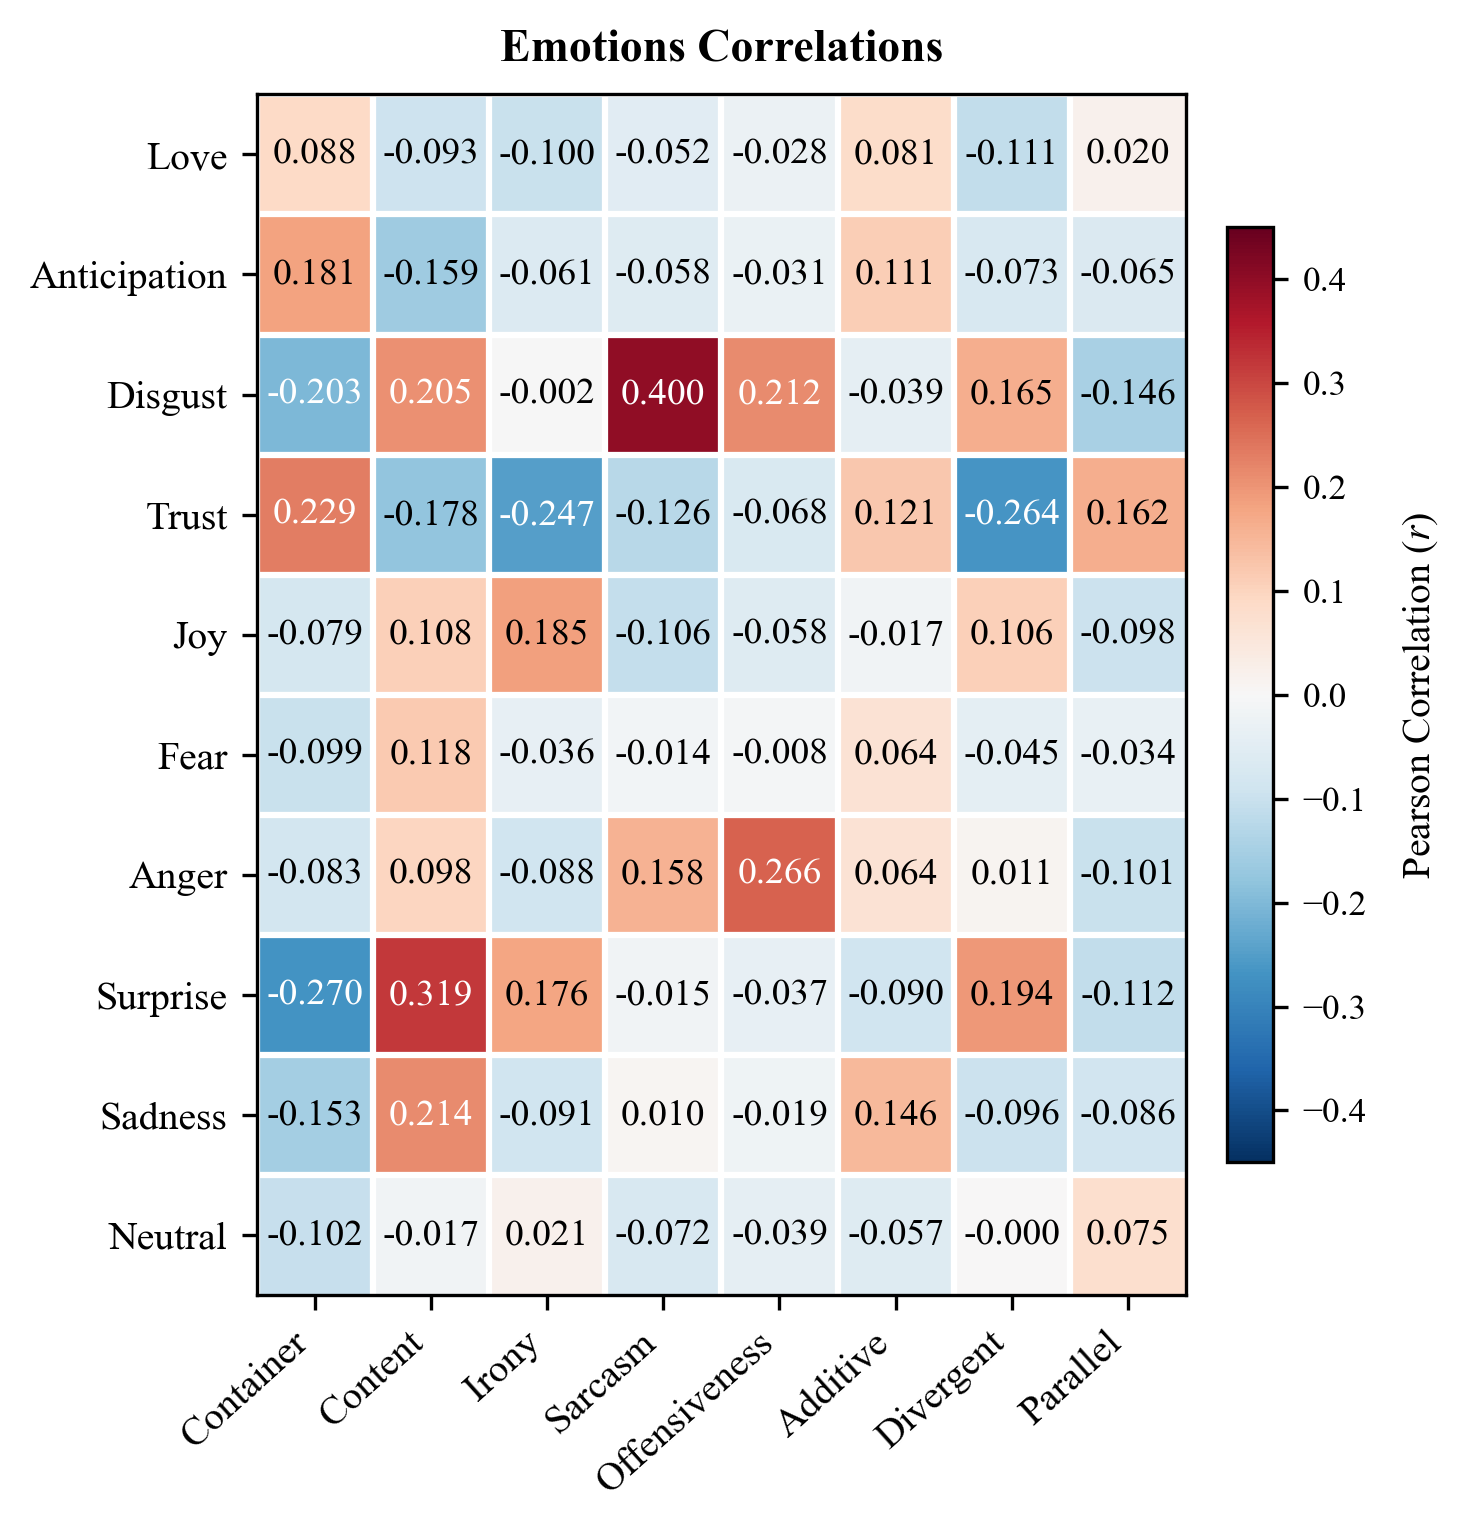
\includegraphics[width=0.92\columnwidth]{imgs/emotion_correlations_english.png}
\caption{Pearson correlation matrix between emotion labels and contextual dimensions (broadcast targets, figurative speech, and semiotic relations) in the Multimodal partition.}
\label{fig:emotions_correlations}
\end{figure}

\begin{figure*}[!t]
\centering
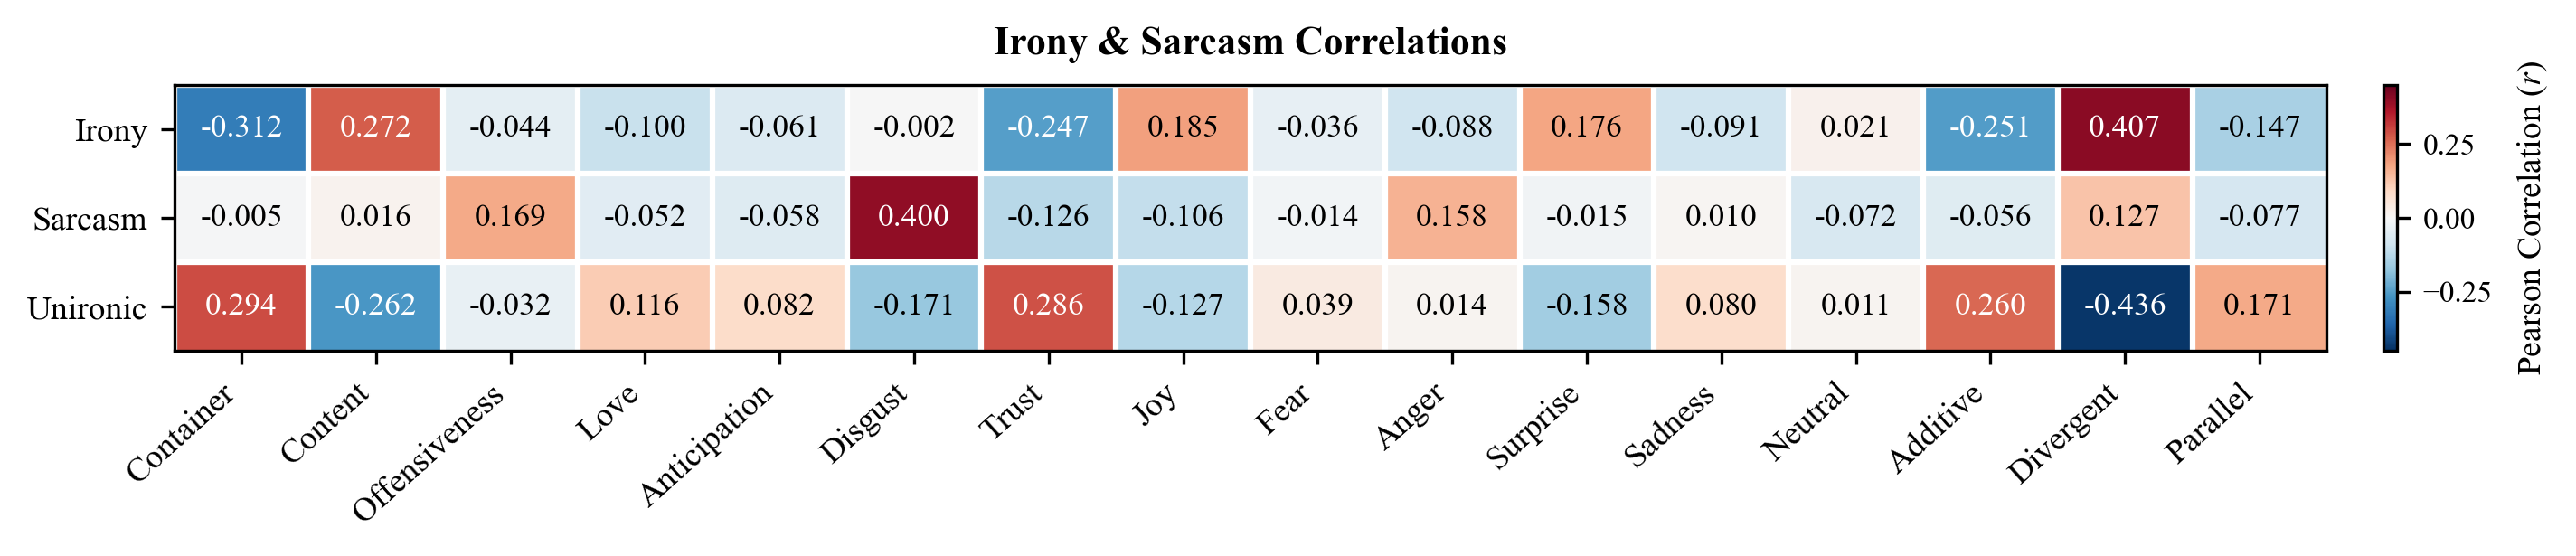
\includegraphics[width=\textwidth]{imgs/irony_correlations_english.png}
\caption{Pearson correlation matrix for the irony and sarcasm dimension across multi-level annotations within the Multimodal partition.}
\label{fig:irony_correlations}
\end{figure*}

\begin{figure*}[!t]
\centering
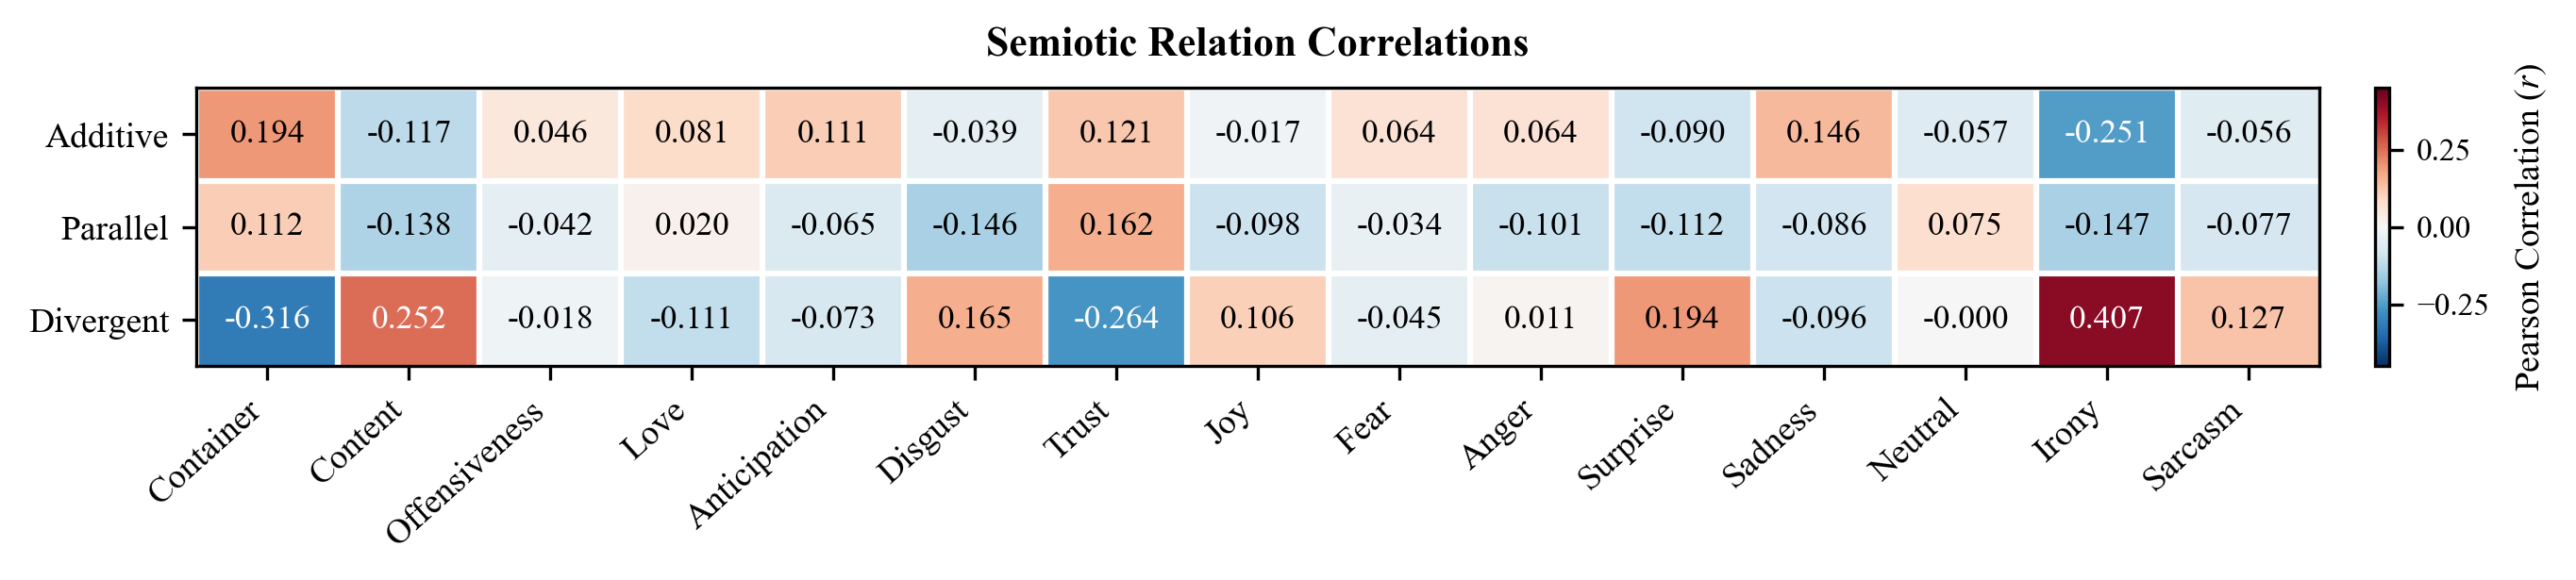
\includegraphics[width=\textwidth]{imgs/relation_correlations_english.png}
\caption{Pearson correlation matrix for semiotic text-image relations against contextual and affective markers in the Multimodal partition.}
\label{fig:relations_correlations}
\end{figure*}

Examining the correlation matrix for \textbf{Emotions} (Fig.~\ref{fig:emotions_correlations}), a clear dichotomy emerges between the \textit{Container} and \textit{Content} targets. Program-directed affective states (\textit{Trust} $r = 0.229$, \textit{Anticipation} $r = 0.181$) correlate positively with Container, indicating audience loyalty toward the show. Conversely, content-reactive emotions (\textit{Surprise} $r = 0.319$, \textit{Sadness} $r = 0.214$, \textit{Disgust} $r = 0.205$) associate with Content. Sarcasm also reveals a hostile pragmatic pattern, correlating positively with \textit{Disgust} ($r = 0.400$), offensive language ($r = 0.169$), and \textit{Anger} ($r = 0.158$).

Analyzing \textbf{Irony} (Fig.~\ref{fig:irony_correlations}), we observe that figurative speech relies fundamentally on semiotic contrast. Irony correlates with \textit{Divergent} text-image relations ($r = 0.407$), the \textit{Content} target ($r = 0.272$), and \textit{Joy} ($r = 0.185$), demonstrating that multimodal irony frequently arises from playful tension between the visual image and the written caption. Sincere posts (\textit{Unironic}), by contrast, correlate with \textit{Container} ($r = 0.294$), \textit{Trust} ($r = 0.286$), and complementary visual relations (\textit{Additive} $r = 0.260$, \textit{Parallel} $r = 0.171$).

Semiotic relations (Fig.~\ref{fig:relations_correlations}) confirm that divergent pairings drive social media irony: Divergent posts correlate positively with \textit{Irony} ($r = 0.407$), \textit{Content} ($r = 0.252$), and \textit{Surprise} ($r = 0.194$). In contrast, the \textit{Additive} relation associates with \textit{Container} ($r = 0.194$) and narrative elaboration, while the \textit{Parallel} relation exhibits minimal correlation with complex emotional states, reflecting literal and redundant text-image usage.